\section{A model for on-the-spot attention and response modulation support in online conversations}~\label{sec:design}
\subsection{Implicit Emotion Regulation}
\subsection{Proposed methodology}
The proposed framework for encouraging emotion regulation in social media conversations is depicted in Figure-\ref{fig:Framework}. It is composed of three key components: data retrieval, emotion propagation analysis, and emotion regulation recommendations. The data retrieval process starts with gathering information from social media conversations, in this case Twitter conversations. In recent years, Twitter has been a popular destination for hashtag-based social movements such as \#MeToo and \#BlackLivesMatter, but the platform's free speech policy also increases the risk of hate and harassment. Therefore, we gathered a variety of Twitter conversations and saved them as CSV files. We used feature engineering to create a set of files, each containing a conversation wherein each row comprised of a text string representing a tweet or a comment, as well as their ID and metadata (parameters like the number of comments received, authors who replied etc). The second component then analyses emotion propagation using these CSV files. It begins with categorising the emotions expressed in tweets. Emotions are divided into 6 primary and 27 secondary groups. We use the primary emotion categories in this work to classify the emotion in tweets. We generate a graph of the conversation after classifying the tweets into 6 emotion classes. This graph is used to calculate the emotional impact of individual tweets on the entire conversation as well as the percentage distribution of various emotions in the discussion. Following that, in the final component, we use the graph to identify the nodes that have the greatest impact on the emotion of the conversation and apply this information to identify scenarios where emotion regulation needs to be undertaken and offer support for the same.
\begin{figure}[h]
  
    \centering
    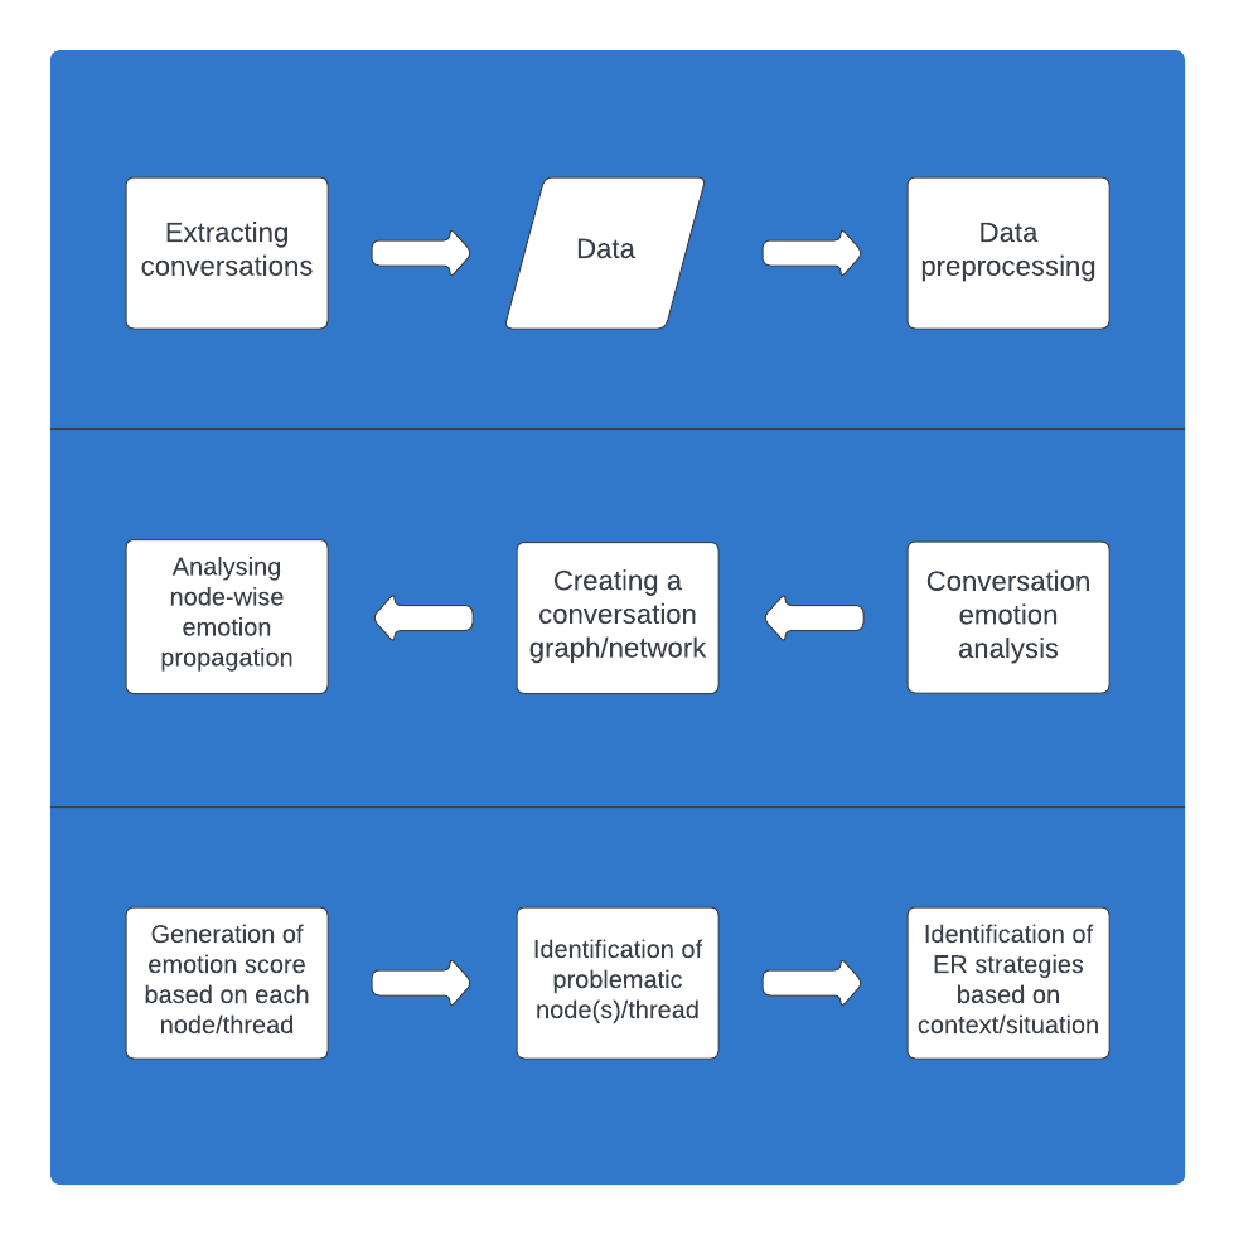
\includegraphics[width=12cm,height=12cm,keepaspectratio]{framework.pdf}
%   \includegraphics[width=5cm,height=5cm,keepaspectratio]{samples/sample_convv.png}
%   \includegraphics[width=5cm,height=5cm,keepaspectratio]{samples/sample_conv_graphh.png}
  \caption{Framework for encouraging on-spot emotion regulation in social media conversations}
  \label{fig:Framework}
  \end{figure}  
%%%%%%%%%%%%%%%%%%%


 

